%------------------------------------------------------------------------
% $Id: exams.tex 1128 2007-07-11 08:55:26Z kaityo $
%------------------------------------------------------------------------
\documentclass{jarticle}

\usepackage{physmath}
\usepackage{graphicx}
\pagestyle{empty}
\newcommand{\diff}{\mathrm d}
\newcommand{\e}{\mathrm e}


\begin{document}

\begin{center}
{\huge 物理数学テストゼミ}\\[3mm]
{\Large 次元解析とテイラー展開}
\end{center}

\question 物理量にはすべて次元(単位)がある。
長さの次元を[L]、時間の次元を$[T]$、質量の次元を$[M]$と表すことにすると、
速さは$[L/T]$、運動量は$[M L/T]$などの
次元を持っている。次元について以下の問いに答えよ。

\subquestion{バネ定数$k$のバネにつながれた、質量$m$の質点がある。
この質点の振動周期$T$は$k$及び$m$だけで決まるであろう。
そこで、
$$
T \sim k^{\alpha} m^{\beta} 
$$
とおいて、次元が合うように$\alpha$、$\beta$の値を決めよ。}

\subquestion{一様重力下(重力加速度$g$)において、質量$m$、長さ$l$の単振り子があるとする。
この振動周波数$\omega$の$m$、$g$、$l$依存性を知りたい。
前問と同様に、
$$
\omega \sim l^{\alpha} m^{\beta} g^{\gamma}
$$
とおいて、次元が合うように$\alpha$、$\beta$、$\gamma$の値を決め、
結果について考察せよ。
}

\question
一様重力下(重力加速度$g$)における質量$m$のボールの運動を考える。
簡単のため、空気抵抗などは無視する。

\subquestion{ボールの運動方程式を立てよ。}
\subquestion{基準の位置からの高さを$y$として、全エネルギーを書け。このとき、
運動エネルギーと位置エネルギーの次元が等しいことを確かめよ。
}
\subquestion{運動方程式から全エネルギーが保存することを確かめよ。}
\subquestion{初速$V_0$とし、仰角$\theta$で地面からボールを投げるとする。
最も遠くに飛ぶ角度を求めよ。}

\question
ある関数$f(x)$を、特定の点$x_0$の近傍で
$$
f(x) = c_0 + c_1(x-x_0) + c_2 (x-x_0)^2 + \cdots 
$$
と展開することを考える(テイラー展開)。
両辺を適当に微分し、$x=x_0$を代入することで係数$c_n$を求めよ。

\question
次の関数を$x=0$の周りでテイラー展開せよ。

\subquestion{$\sin x$ }
\subquestion{$\cos x$ }
\subquestion{$\ln (1+x)$ }

\question
$\sin x$を$x=0$の周りで、$x$について1次まで展開した場合と
3次まで展開した場合で、どの程度近似の程度が異なるか、$0 \le x \le \pi$の範囲で
グラフに描いて考察せよ。特に$x = \pi/2$を代入した場合の値の違いを見よ。


%-----------------------------------------------------------------------
\newpage
%-----------------------------------------------------------------------

\begin{center}
{\huge 物理数学テストゼミ}\\[3mm]
{\Large 微分方程式の解法}
\end{center}

\question 微分方程式のうち、一種類の変数のみによる微分しか含まないものを
常微分方程式と呼ぶ。以下の常微分方程式の一般解を求めよ。

\subquestion{
$$\frac{\diff y}{\diff x} = \frac{\ln x}{y} $$
}

\subquestion{
$$\frac{\diff y}{\diff x} + y= 2 \sin x $$
}

\subquestion{
$$\frac{\diff^2 y}{\diff x^2} + 3 \frac{\diff y}{\diff x} + 2y = 0 $$
}

\question 微分方程式に含まれる定数は、初期条件などを与えることで
定まる。これを初期値問題(境界値問題)と呼ぶ。次の初期値問題の解を求めよ。
また$x>0$における解の振る舞いを描け。

\subquestion{
$$\frac{\diff^2 y}{\diff x^2} + 4 \frac{\diff y}{\diff x} + 3y = 0
\qquad y(0) = 0,  \left. \frac{\diff y}{\diff x} \right|_{x=0} = 1
$$
}

\subquestion{
$$\frac{\diff^2 y}{\diff x^2} + 2 \frac{\diff y}{\diff x} + 2y = 0
\qquad y(0) = 1, \left. \frac{\diff y}{\diff x} \right|_{x=0} = 0
$$
}

\question 微分方程式のうち、独立な二変数以上の微分を含むものを偏微分方程式と呼ぶ。
偏微分方程式について以下の問いに答えよ。

\subquestion{
$t$と$x$の関数$u(x,t)$について、以下の偏微分方程式の一般解を求めよ(ただし$\kappa >0$)。
$$ \frac{\partial u}{\partial t} =  \kappa \frac{\partial^2 u}{\partial x^2} $$
}

\subquestion{
前問で、固定境界条件$u(0,t) = u(\pi,t) = 0$を与えた場合の特殊解を求めよ。
}

\question 上記の微分方程式は、ほぼすべて線形(linear)方程式であった。
線形とは、$f_1$、$f_2$が方程式の解であるとき、その線形和 $a f_1 + b f_2$も解であるような
性質である($a,b$は定数)。以下の方程式は線形か確認せよ。

\subquestion{
$$ \frac{\partial u}{\partial t} +  \frac{\partial^3 u}{\partial x^3} + 6  \frac{\partial u}{\partial x}  = 0$$
}
\subquestion{
$$ \frac{\partial u}{\partial t} +  \frac{\partial^3 u}{\partial x^3} + 6  u \frac{\partial u}{\partial x}  = 0$$
}

%-----------------------------------------------------------------------
\newpage
%-----------------------------------------------------------------------

\begin{center}
{\huge 物理数学テストゼミ}\\[3mm]
{\Large 基底と固有値問題}
\end{center}

\question 行列$A$とベクトル${\bf x}$について、$A {\bf x} = \lambda {\bf x}$が
成り立つとき、${\bf x}$を$A$の固有ベクトル、$\lambda$を固有値と呼ぶ。
行列
$
A = \left(
\displaystyle\begin{array}{cc}
1 & -2 \\
-2 & 1
\end{array}
\right)
$
について以下の問いに答えよ。

\subquestion{
行列の固有値、及び対応する規格化された固有ベクトルを求めよ。
ここで求められた固有ベクトルは互いに直交しているか確認せよ。
}

\subquestion{
前問で求めた固有ベクトルをそれぞれ${\bf e}_1,{\bf e}_2$とする。
ベクトル${\bf a} =  \displaystyle
\left(
\begin{array}{c}
3 \\ 4
\end{array}
\right)
$
を、
$$
{\bf a} = c_1 {\bf e}_1 +c_2 {\bf e}_2
$$
と展開することを考える。$c_1, c_2$を求めよ。
}

\subquestion{
得られた固有ベクトルを用いて行列$A$を対角化せよ。
その結果を用いて$A^n$を求めよ。
}

\question 
ハミルトニアン$\cal H$に対し、関数$\psi$が${\cal H}\psi = E \psi$を満たすとき、
$\psi$を波動関数、$E$をエネルギー固有値という。この波動関数とエネルギー固有値を
求める問題も固有値問題と呼ぶ。固有値問題の例として、
時間を含まない一次元シュレーディンガー(Schr\"odinger)方程式、
$$
 \left( -\frac{\hbar^2}{2m} \frac{\diff^2}{\diff x^2} + V(x) \right) \psi = E \psi
$$
を考えよう。$V(x)$はポテンシャルを表す。$m$、$\hbar$、$E$は
いずれも正の実数とする。

\subquestion{ ポテンシャル$V(x)=0$の場合、$\psi(x)$の一般解を求めよ。}

\subquestion{ 一次元$-L/2<  x < L/2$の範囲で自由に運動する粒子が従う
規格化された波動関数$\psi$を求めよ。また、対応するエネルギー固有値も求めよ。
}

\subquestion{前問で求めた波動関数について、
異なるエネルギー固有値に対応する波動関数が互いに直交することを示せ。
}

\question 前問のポテンシャルとして、$V(x) = m \omega^2 x^2/2$を考える。
これは原点からの距離の二乗でエネルギーが高くなる、調和振動子を表している。
この系について以下の問いに答えよ。

\subquestion{ 基底状態の波動関数を$\psi_0(x) = N_0 \exp{(-a^2 x^2/2)} $とおいて
代入し、これが解であることと規格化条件から$a$、$E$、$N_0$を求めよ。
}

\subquestion{ この方程式の一般解は Hermiteの多項式 $H_n(x)$を用いて
$$
\psi_n(x) = N_n H_n(ax) \exp{(-a^2 x^2/2)} 
$$
と表すことができる。$H_n(ax)$の満たすべき微分方程式を求めよ。
(ヒント: $ax \rightarrow \xi$と変数変換し、前問で求めた$a$を代入すると微分方程式が簡単な形になる)
}

\subquestion{
Hermiteの多項式は、具体的には$H_0 = 1$、$H_1 = 2x$、$H_2 = 4x^2-2$
である。$\psi_0(x)$と$\psi_1(x)$、$\psi_2(x)$がそれぞれ直交していることを
確かめよ。
}


%-----------------------------------------------------------------------
\newpage
%-----------------------------------------------------------------------

\begin{center}
{\huge 物理数学テストゼミ}\\[3mm]
{\Large フーリエ級数展開と超関数}
\end{center}

\question
$(-\pi \le x < \pi)$で定義されている関数$f(x)$を、
$$
f(x) = \frac{a_0}{2} + \sum_{n=1}^\infty (a_n \cos nx + b_n \sin nx)
$$
の形に展開することをフーリエ級数展開という。以下の関数を
フーリエ級数展開せよ。また、$x=0$を代入して値が正しいか確認せよ。

\subquestion{
$f(x) = |x|$
}

\subquestion{
$f(x) = 
\left\{
\begin{array}{cc}
-1 & \quad -\pi \le x < 0 \\
1 & \quad 0 \le x \le \pi 
\end{array}
\right.
$
}

\question
$(-\pi \le x < \pi)$で定義されている関数$f(x)$を、
$$
f(x) = \sum_{-\infty}^{\infty} c_n \exp{(inx)}
$$
の形に展開することを複素フーリエ級数展開という($c_n$は複素数)。
これについて以下の問いに答えよ。

\subquestion{フーリエ級数展開と、複素フーリエ級数展開を比べ、
$c_n$を$a_n$、$b_n$で表せ。
}

\subquestion{
$ f(x) = \mathrm{e}^x ~(-\pi \le x < \pi)$ を複素フーリエ級数展開し、
この結果を用いて、
$
\displaystyle
\sum_{n=1}^{\infty} \frac{(-1)^n}{1+n^2}
$ の値を求めよ。
}

\question 
次の積分で定義される関数$\delta(x)$を、ディラック(Dirac)のデルタ関数という。
$$
\int_{-\infty}^{\infty} \!\!\! \diff x \delta(x) f(x) =
\int_{-\varepsilon}^{\varepsilon} \!\!\! \diff x \delta(x) f(x) = 
f(0)
$$
ただし$\varepsilon$は任意の正数である。また、
次のような関数$\theta(x)$を階段関数、もしくはヘビサイド(Heaviside)関数という。
$$
\theta(x) = 
\left\{
\begin{array}{cc}
0 & \quad (x < 0) \\
1 & \quad (x \ge 0) \\
\end{array}
\right.
$$
これらの関数について、以下の問いに答えよ。
ただし、デルタ関数、ヘビサイド関数と内積をとる関数$f(x)$は、
$f(\infty) = f(-\infty) = 0$であり、何回でも微分ができる性質を持つものとする。

\subquestion{次の等式を証明せよ。
\begin{eqnarray*}
x \delta(x) &=& 0\\
\delta(ax) &=& \delta(x)/|a|, ~(a \neq 0)
\end{eqnarray*}
}

\subquestion{次の等式を証明せよ。
$$
\displaystyle\frac{\diff \theta(x)}{\diff x} = \delta(x)
$$
}

\subquestion{ デルタ関数$\delta(x)$を、$(-\pi \le x < \pi)$の範囲で定義されていると考えて
複素フーリエ級数展開せよ。
}

%-----------------------------------------------------------------------
\newpage
%-----------------------------------------------------------------------

\begin{center}
{\huge 物理数学テストゼミ}\\[3mm]
{\Large フーリエ変換}
\end{center}

\question{関数$f(x)$について、
$$
\hat{f}(k) = \int_{-\infty}^{\infty} \!\!\! \diff x f(x) \e^{-ikx}
$$
をフーリエ変換と呼び、$\hat{f}(k) = {\cal F}[f(x)]$とあらわす。また、
$$
f(x) = \frac{1}{2\pi} \int_{-\infty}^{\infty} \!\!\! \diff k \hat{f}(k) \e^{ikx}
$$
を逆フーリエ変換$(f(x) = {\cal F}^{-1}[\hat{f}(k)])$と呼ぶ。
この時、以下を証明せよ。ただし、
$f^{(n)}(\pm \infty)=0$とする。
}

\subquestion{%
${\cal F}\left[ a f(x) + b g(x) \right] = a{\cal F}[f(x)] + b{\cal F}[g(x)]$\qquad(線形性)
}

\subquestion{%
${\cal F}\left[f^{(n)}(x) \right] = (ik)^n \hat{f}(k)$
}

\subquestion{%
${\cal F}[f(x+a)] = \e^{iak}\hat{f}(k)$
}

\subquestion{%
${\cal F}[x^n f(x)] = i^n \hat{f}^{(n)}(k)$
}

\subquestion{%
${\cal F}[f*g(x)] = {\cal F}[f(x)] {\cal F}[g(x)] $\\
ただし、$f*g(x)$は
$$
f*g(x) = \int_{-\infty}^{\infty} f(x-y)g(y)\diff y
$$
で定義される積分である(たたみ込み積分と呼ばれる)。
}


\question{%
次の関数のフーリエ変換を求めよ。ただし$a>0$とする。
}

\subquestion{%
$$
f(x) = 
\left\{
\begin{array}{cc}
1 & \qquad |x| \le a \\
0 & \qquad |x| > a \\
\end{array}
\right.
$$
}
\subquestion{%
$$f(x) = \e^{-a|x|}$$
}

\question{%
次の微分方程式を満たす解を$y(x)$、そのフーリエ変換を$\hat{y}(k)$とする。
方程式全体をフーリエ変換することで$\hat{y}(k)$を求めよ。
}
\subquestion{%
$$\frac{\diff^2 y}{\diff x^2} - 2 \frac{\diff y}{\diff x} = \delta(x)$$
}
\subquestion{%
$$\frac{\diff^2 y}{\diff x^2} - y = \e^{-ax^2} \qquad (a>0)$$
}


%-----------------------------------------------------------------------
\newpage
%-----------------------------------------------------------------------

\begin{center}
{\huge 物理数学テストゼミ}\\[3mm]
{\Large 複素積分とローラン展開}
\end{center}

\question{%
複素関数$f(z)$が点$z_0$で微分可能であるとは、
$\lim z \rightarrow z_0$へどのように近づいても極限
$$
\lim_{\Delta z \rightarrow 0} \frac{f(z+\Delta z) - f(z)}{\Delta z}
$$
が同じ値に定まることである(ただし$\Delta z = z - z_0$)。
このとき、複素関数の微分について以下の問に答えよ。
ただし、複素数$z$を二つの実数を用いて$z = x + iy$と、
複素関数$f(z)$を、二つの実数関数を用いて$f(z) = u(x,y) + i v(x,y)$と表す。
}

\subquestion{%
$f(z)$が微分可能であるとき、$u(x,y)$と$v(x,y)$が、以下の関係式
$$
\frac{\partial u}{\partial x} = \frac{\partial v}{\partial y},
\frac{\partial u}{\partial y} = -\frac{\partial v}{\partial x},
$$
を満たすことを示せ。
この関係式をコーシー・リーマン(Cauchy-Riemann)の関係式という。
}

\subquestion{%
複素関数$f(z) = z^2$はコーシー・リーマンの関係式が成り立つか確認せよ。
}

\subquestion{%
複素関数$f(z) = z \bar{z}$はコーシー・リーマンの関係式を満たすか確認せよ。
ただし$\bar{z}$は$z$の複素共役を表す。
}

\question{%
複素関数が$f(t) = u(t) + i v(t)$とパラメータ$t$で表示されるとき、
$f(t)$の区間$[a,b]$での定積分を
$$
\int_a^b f(t) \diff t = \int_a^b  u(t)\diff t + i \int_a^b  v(t) \diff t
$$
で定義する。このとき、以下の積分を求めよ。
ただし、括弧内は積分区間である。
}

\subquestion{%
$f(z) = z^2$ (原点$0$から点$1+i$にいたる線分)
}

\subquestion{%
$f(z) = (z-a)^n ~(n = 0,\pm 1, \pm 2,\cdots)$ (点$a$を中心とする半径$r (>0)$の円周上を反時計周りに一周)。
}

\question{%
関数$f(z)$が領域$D$において微分可能であるとき、関数$f(z)$は$D$において
正則であるという。点$a$が$f(z)$の孤立特異点であり、
$f(z)が$領域$D = \{ z | r_1 < |z-a|  <r_2 \}$において正則であるとき、
$f(z)$は点$a$の周りで
$$
f(z) = \sum_{-\infty}^{\infty} c_n (z-a)^n
$$
と展開される。これを$f(x)$の$a$におけるローラン(Laurent)展開と呼ぶ。
このとき、以下の問に答えよ。
ヒント:収束半径$(|z|<1)$に注意して以下の展開を利用せよ。
$$
\frac{1}{1+z} = 1-z+z^2-\cdots + (-1)^n z^n + \cdots \quad 
$$
}

\subquestion{%
$f(z) = \displaystyle\frac{1}{z-1}$を原点を中心とし、$|z|<1$及び$1<|z|$のそれぞれの
場合についてローラン展開せよ。
}

\subquestion{%
$f(z) = \displaystyle\frac{1}{z(z-1)}$を原点を中心とし、$|z|<1$及び$1<|z|$のそれぞれの
場合についてローラン展開せよ。
}

%-----------------------------------------------------------------------
\newpage
%-----------------------------------------------------------------------

\begin{center}
{\huge 物理数学テストゼミ}\\[3mm]
{\Large 留数定理とその応用}
\end{center}

\question{%
関数$f(z)$は領域$D$で正則であり、
$C$は領域$D$内の単一閉曲線であるとする。
このとき、$C$内の点$a$について、以下の公式が成り立つ(コーシーの積分公式)。
$$
f(a) = \frac{1}{2\pi i} \int_C \frac{f(z)}{z-a} \diff z
$$
これを用いて次の積分の値を求めよ。
}

\subquestion{%
$
 \displaystyle \int_{|z|=2} \frac{\e^z}{z+1} \diff z \quad \mbox{(原点を中心とし、半径$2$の円を正の向きに一周する積分路を表す。以下同様 )}
$
}

\subquestion{%
$
\displaystyle \int_{|z|=2}  \frac{z}{z^2+1} \diff z
$
}

\question{%
関数$f(z)$は領域$D$で正則であり、
$C$は領域$D$内の単一閉曲線であるとする。
このとき、$C$内の点$a$について、以下の公式が成り立つ(これもコーシーの積分公式)。
$$
f^{n}(a) = \frac{n!}{2\pi i} \int_C \frac{f(z)}{(z-a)^{n+1}} \diff z
$$
これを用いて次の積分の値を求めよ。
}

\subquestion{%
$
 \displaystyle \int_{|z|=3} \frac{\e^{3z}}{(z-2)^2} \diff z 
$
}

\subquestion{%
$
\displaystyle  \int_{|z|=1}  \frac{1}{z^2(z-3)} \diff z
$
}

\question{%
関数$f(z)$が、$z=a$を孤立特異点として持つとき、
$$
\mbox{Res}f(a) \equiv \frac{1}{2\pi i} \int_C f(z) \diff z
$$
を$f(z)$の$a$における{\bf 留数 (residue)}と呼ぶ(ただし$C$は$a$の近傍を正の方向に一周する積分路とする)。
以下の関数のすべての特異点における留数を求めよ。
}

\subquestion{%
$
\displaystyle \frac{\e^{iz}}{z^2+a^2} \qquad (a > 0)
$
}

\subquestion{%
$
\displaystyle \frac{1}{z^4+1}
$
}

\question{%
次の実積分の値を、複素積分を利用して求めよ。
}

\subquestion{%
$
\displaystyle \int_{0}^{\infty} \frac{1}{x^4+1} \diff x
$
}

\subquestion{%
$
\displaystyle \int_{-\infty}^{\infty} \frac{\cos k x}{x^2+1} \diff x \qquad (k>0)
$
}

%-----------------------------------------------------------------------
\newpage
%-----------------------------------------------------------------------

\begin{center}
{\huge 物理数学テストゼミ}\\[3mm]
{\Large フーリエ逆変換とジョルダンの補題}
\end{center}

\question{$\displaystyle\lim_{|z| \rightarrow \infty} f(z) = 0$を満たす複素関数$f(z)$を考える。
このとき、ある実数$a>0$について、積分路を以下の図の$C_1$のように取ると、
$$
\lim_{R \rightarrow \infty} \int_{C} f(z)\e^{iaz} = 0
$$
が成り立つ(ジョルダンの補題)。$a<0$のときは$C_2$のように取れば、同様に成り立つ。
このことに注意して、以下の問いに答えよ。
}

\begin{figure}[htbp]
\begin{center}
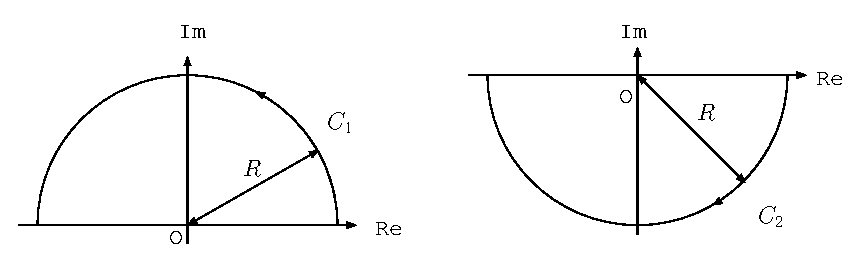
\includegraphics[width=.6\linewidth]{fig/jordan.eps}
\end{center}
\end{figure}

\subquestion{
以下の関数$f(x)$をフーリエ変換せよ。ただし$a>0$とする。
$$
f(x) = \left\{
\begin{array}{cc}
1 & \quad (-a < x < a) \\
0 & \mbox{otherwise}
\end{array}
\right.
$$
}

\subquestion{
前問で求められたフーリエ変換$\hat{f}(k)$を逆フーリエ変換し、
$f(x)$に一致することを確かめよ。\\
ヒント:$x<-a$、$-a \leq x < a$、$a \leq x $の場合にわけて
積分路を考えよ。
}

\question{次の微分方程式の境界値問題を以下の手順で解け。
$$
\frac{\diff^2 f(x)}{\diff x^2} - f(x) = \e^{-|x|} \qquad f(\pm \infty) = f'(\pm \infty)=0
$$
}

\subquestion{
微分方程式全体をフーリエ変換せよ。
}

\subquestion{
逆フーリエ変換により、解を求めよ。\\
ヒント:$x>0$と$x<0$に場合わけすること。
}

\subquestion{
解を微分方程式に代入し、実際に解であることを確かめよ。
}

%-----------------------------------------------------------------------
\newpage
%-----------------------------------------------------------------------

\begin{center}
{\huge 物理数学テストゼミ}\\[3mm]
{\Large ラプラス変換}
\end{center}


\question{関数$f(x)$について、
$$
\hat{f}(s) = \int_{0}^{\infty} \!\!\! \diff x f(x) \e^{-sx}
$$
をラプラス変換と呼び、$\hat{f}(s) = {\cal L}[f(x)]$とあらわす。
ただし、$s$はラプラス変換が存在するように値をとった複素数である。このとき、以下を証明せよ。
}

\subquestion{%
${\cal L}\left[f^{(n)}(x) \right] = s^n \hat{f}(s) - \left\{ s^{n-1}f(0) + s^{n-2}f'(0) + \cdots  \right\} $
}

\subquestion{%
${\cal L}\left[\e^{ax}f(x) \right] = \hat{f}(s-a)$
}


\subquestion{%
${\cal L}[f*g(x)] = {\cal L}[f(x)] {\cal L}[g(x)] $\\
ただし、$f*g(x)$は
$$
f*g(x) = \int_{0}^{x} f(x-y)g(y)\diff y
$$
で定義される積分である(たたみ込み積分と呼ばれる)。
}

\question{次の関数$f(x)$のラプラス変換を求めよ。
必要であればラプラス変換が存在するための$s$の条件も求めよ。
}

\subquestion{
$
f(x) = 1
$
}

\subquestion{
$
f(x) = \delta(x)
$
}

\subquestion{
$
f(x) = x
$
}

\subquestion{
$
f(x) = \e^{\alpha x} \quad (\mbox{$\alpha$は複素定数})
$
}

\question{関数$f(x)$とそのラプラス変換$\hat{f}(s)$について、
$s = a + bi$とするとき
$$
f(x) = \frac{1}{2 \pi i} \int_{a-i\infty}^{a+i\infty} \diff s \hat{f}(s) \e^{sx}
$$
を逆ラプラス変換と呼ぶ。以下の関数を逆ラプラス変換せよ。
}

\subquestion{
$\hat{f}(s) = \displaystyle \frac{1}{s-\alpha}  \qquad {\mbox{$\alpha$は複素定数}}$
}

\subquestion{
$\hat{f}(s) =  \displaystyle\frac{s}{s^2+c^2}  \qquad {\mbox{$c$は実定数}}$
}

\question{以下の微分方程式の初期値問題をラプラス変換を用いて解け。
}

\subquestion{%
$
\displaystyle\frac{\diff^2 y}{\diff x^2} - 2\frac{\diff y}{\diff x} + y = x
\qquad \left( y(0) = y'(0) = 0 \right)
$
}

\subquestion{%
$
\displaystyle\frac{\diff^2 y}{\diff x^2} + 2\frac{\diff y}{\diff x} + y = 1
\qquad \left( y(0) = y'(0) = 0 \right)
$
}

\end{document}
